\documentclass{article}
\usepackage{graphicx,fancyhdr,amsmath,amssymb,amsthm,subfig,url,hyperref}
\usepackage[margin=1in]{geometry}

\usepackage{natbib}
\usepackage{cancel}

\usepackage{minted}

%----------------------- Macros and Definitions --------------------------

%%% FILL THIS OUT
\newcommand{\studentname}{Jane Doe}
\newcommand{\suid}{janedoe}
\newcommand{\exerciseset}{Homework}
%%% END



\renewcommand{\theenumi}{\bf \Alph{enumi}}

\theoremstyle{plain}
\newtheorem{theorem}{Theorem}
\newtheorem{lemma}[theorem]{Lemma}


\graphicspath{{figures/}}

%-------------------------------- Title ----------------------------------

\title{Study Kasus 1: Implementasi Algoritma Luhn}
\author{IN232 Matematika Diskrit}
\date{}
%--------------------------------- Text ----------------------------------

\begin{document}
\maketitle

\section*{Latar Belakang}
Umumnya, nomor kartu kredit memiliki 13, 15, atau 16 digit. Sebagai contoh,
\begin{equation}
	4690 3582 1375 4657
	\label{eq:contoh-nomor-kartu-kredit}
\end{equation}
merupakan nomor kartu kredit rekaan. Digit pertama menunjukkan sistem. Dalam nomor kartu kredit di Persamaan \eqref{eq:contoh-nomor-kartu-kredit}, digit pertama, 4, menunjukkan bahwa kartu tersebut adalah kartu Visa. Digit berikut menunjukkan informasi lain seperti nomor rekening dan nomor bank. (Penjelasan tepatnya tergantung pada jenis kartunya.) Digit terakhir adalah spesial karena digit tersebut dihitung dari digit sebelumnya dan disebut digit cek (\textit{check digit}). Dalam Persamaan \eqref{eq:contoh-nomor-kartu-kredit}, digit cek adalah 7 dan nilai ini dihitung dari digit sebelumnya 4690 3582 1375 465. Digit cek kartu kredit digunakan untuk mengidentifikasi apakah nomor kartu kredit tersebut benar atau salah. Alasan penggunaan digit cek bukan untuk alasan keamanan, melainkan digit cek itu digunakan untuk membantu mendeteksi kesalahan seperti ketika seseorang memberikan nomor kartu kredit melalui telepon dan digit cek digunakan untuk mendeteksi apakah nomor kartu kredit yang diberikan tersebut benar atau salah \citep{johnsonbaugh2009discrete}.

Digit cek dihitung sebagai berikut. Mulai dari digit paling kanan; digit ini adalah digit cek dan kita skip digit ini. Gandakan setiap nomor lainnya. Jika hasil penggandaan adalah merupakan bilangan berdigit dua, tambahkan kedua digit tersebut menjadi satu angka; jika bukan bilangan berdigit dua, gunakan digit apa adanya.

\begin{figure}[!ht]
	\centering
	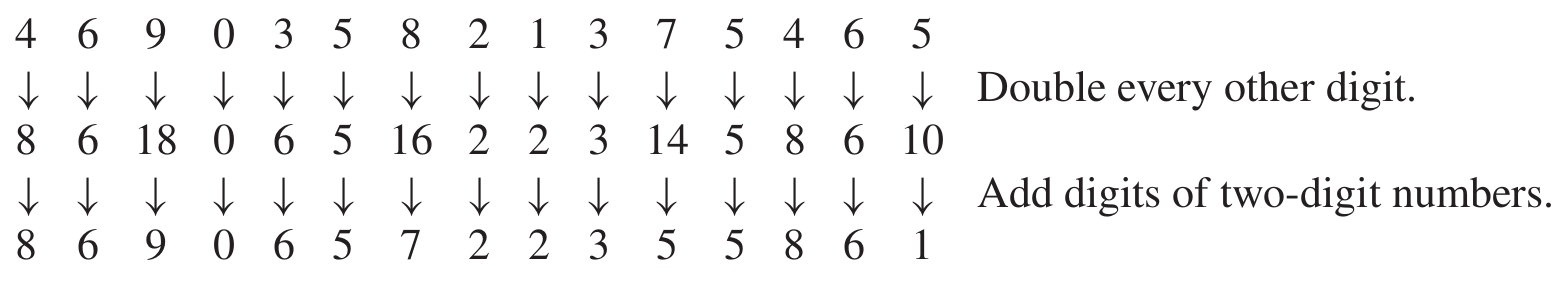
\includegraphics[scale=.25]{images/contoh-perhitungan-luhn}
	\caption{Contoh perhitungan algoritma Luhn}
	\label{fig:contoh-perhitungan-luhn}
\end{figure}

\noindent Jumlahkan angka yang dihasilkan

\begin{equation*}
	8+6+9+0+6+5+7+2+2+3+5+5+8+6+1 = 73.
\end{equation*}

Jika digit terakhir dari penjumlahan adalah 0, digit cek adalah 0. Jika digit terakhir bukan 0, kurangi 10 dengan digit terakhir untuk mendapatkan digit cek, contoh kasus di atas adlaah $10 - 3 = 7$. Verifikasi digit cek pada kartu Visa, MasterCard, American Express, atau Diners Club favorit anda. Cara menghitung cek digit ini disebut \textit{Algoritma Luhn}. Algoritma ini diciptakan oleh Hans Peter Luhn (1896-1964), yang menciptakannya saat di beliau bekerja di IBM. Meskipun awalnya dipatenkan, sekarang aloritma ini  digunakan secara luas di domain publik.

\section*{Implementasi}
Tugas anda adalah mengimplementasi Algoritma Luhn di dalam method 

\begin{minted}{python}
def compute_check_digit(a_number):
    """
    Compute a check digit from a sequence of credit card number by employing Luhn algorithm	
    
    Parameters:
    -----------
    a_number : int
        A credit card number. For example, 4690358213754657
    
    Returns:
    --------
    check_digit : int
        A digit between 0 dan 9 inclusively. 
    """
    pass
\end{minted}

\noindent Sebagai test drive, anda dapat coba memanggil
\begin{minted}{python}
compute_check_digit(469035821375465) # 7
compute_check_digit(469035827375465) # 4
\end{minted}


\bibliographystyle{apalike}
\bibliography{references}


\end{document}
